\chapter{MBDyn and Airframe Modeling}
\label{ch:chapter1}

This chapter introduces the fundamental principles of MBDyn, a multibody dynamics software package. The key setup of the MBDyn program is discussed, followed by an overview of the relevant MBDyn modules essential for modeling an airframe. Finally, the chapter delves into the specific steps involved in constructing and verifying the accuracy of the airframe model.

\section{MBDyn Software Simulator}
This research utilizes MBDyn, a free multibody dynamics software developed by the Department of Aerospace Engineering (DIAPM) at Politecnico di Milano, Italy. MBDyn offers inherent capabilities for external communication through both local and network configurations. This communication is facilitated by internet and Unix domain sockets, acting as bidirectional communication endpoints at the kernel level. The Stream driver function within MBDyn enables this communication.

Based on the works in \cite{battaini2020}, \cite{martello2021}, and \cite{battaini2022}, the structure of the airframe in \cite{martello2021} was used to build the flight equations of motion with kinematic and dynamic equations in \textit{Simulink} software. Furthermore, a control system was developed for both multi-copter mode and fixed-wing mode. Due to the limitations of the simplified equations of motion, it is challenging to simulate the real conditions of vehicle flight in complex environments. Current airframe modeling schemes may not fully capture the complexities of real-world systems. This necessitates the development of more advanced approaches to achieve more realistic simulations.

MBDyn provides a valuable alternative for simulating the airframe, potentially leading to more realistic results compared to traditional methods \cite{Migliore2019}. This enhanced realism stems from MBDyn's ability to model complex interactions within the airframe. However, the control system design will follow the approach outlined in the references, utilizing \textit{Simulink} for further analysis of drone maneuver performance in subsequent chapters. This choice leverages the extensive analysis tools offered by MATLAB. It is important to note that alternative software could be employed for the control system design to avoid dependence on commercial software.

\subsection{Unconstrained Dynamics}
Because the airframe can move freely in all six degrees of freedom (DoF), the equations governing its motion are described as unconstrained dynamics. We can derive the equations of motion (EOMs) for this unconstrained system using the well-established Newton-Euler approach.

The equations of motion (EOMs) of a general mechanical system are usually derived by the Newton-Euler approach. For a system of unconstrained bodies, EOMs are described by:

\begin{equation}
     M(q) \ddot{q} = l(q, \dot{q}, t)  \label{eq:4_1_1}
\end{equation}

\( l(q, \dot{q}, t) \) is the function describing the external forces acting on nodes and may include structural deformability contributions.

Written in the form of a first-order system, equation \ref{eq:4_1_1} becomes:

\begin{equation}
    M(q) \dot{q} = p \label{eq:4_1_2a}
\end{equation}
\begin{equation}
    \dot{p} = l(q, \dot{q}, p, t) \label{eq:4_1_2b}
\end{equation}

where \( p \in \mathbb{R}^n \) is the momenta and momentum moments vector.

\subsection{Constrained Dynamics}

There exist two types of constraints, holonomic and non-holonomic. Both are modeled by adding explicit algebraic relations:

\textbf{Holonomic Constraints:}
\begin{equation}
    0 = \Phi(q, t) \label{eq:4.1.3}
\end{equation}

\textbf{Non-holonomic Constraints:}
\begin{equation}
    0 = \Psi(q, \dot{q}, t)) \label{eq:4.1.4}
\end{equation}

By using Lagrange’s multipliers formalism, system \ref{eq:4_1_2b} becomes:
\begin{equation}
    M(q) \dot{q} = p ) \label{eq:4.1.5a}
\end{equation}
\begin{equation}
    \dot{p} + \Phi^T/q\lambda + \Psi^T/\dot{q}\mu = l(q, \dot{q}, p, t) \label{eq:4.1.5b}
\end{equation}
\begin{equation}
    \Phi(q, t) = 0 \label{eq:4.1.5c}
\end{equation}
\begin{equation}
    \Psi(q, \dot{q}, t) = 0 \label{eq:4.1.5d}
\end{equation}

where \( \lambda \) and \( \mu \) are the Lagrange’s multipliers.

\section{Numerical Integration}
MBDyn's analyses are based on a unique formulation for the direct time integration of initial value problems (IVPs). These IVPs are expressed as a system of first-order differential-algebraic equations (DAEs) and are solved using implicit, nearly L-stable integration algorithms.

Numerical integration is a fundamental computational technique used to approximate solutions for ordinary differential equations (ODEs) or DAEs. In systems where analytical solutions are impractical, numerical integration plays a crucial role in simulating dynamic behavior across various fields, including engineering and physics.

The Differential Algebraic Equation (DAE) system \ref{eq:4_1_2b} has the general form:

\begin{equation}
    h(\dot{x}, x, t) = 0 \label{eq:4.1.6}
\end{equation}

where \( x = (q, p, \lambda, \mu)^T \).

The numerical solution at time \( t_{k+1} \) using the general multistep method is obtained by solving equation \ref{eq:4.1.6} for \( \dot{x}_{k+1} \) with:

\begin{equation}
    x_{k+1} = \sum_{j=0}^{p-1} (a_j x_{k-j} + h b_j \dot{x}_{k-j}) + h b_p \dot{x}_{k+1} \label{eq:4.1.7}
\end{equation}

Using a Newton-Raphson scheme, the solution is given by:

\begin{equation}
    h_{/\dot{x}} \delta \dot{x}_{k+1} + h_{/ x} \delta x_{k+1} = -h  \label{eq:4.1.8}
\end{equation}

Inserting equation \ref{eq:4.1.7} into equation \ref{eq:4.1.8} yields:

\begin{equation}
    \left(h_{/ \dot{x}} + h b_p h_{/ x}\right) \delta \dot{x}_{k+1} = -h \label{eq:4.1.9}
\end{equation}

because:

\begin{equation}
    \delta x_{k+1} = h b_p \delta \dot{x}_{k+1} \label{eq:4.1.10}
\end{equation}

For each time step (that is, for each instant \( t_k \) of the time grid), iterations are performed to solve equation \ref{eq:4.1.9} until convergence is reached.

\subsection{Two-Step BDF Method}
The Two-Step BDF method is a specific variant of the Backward Differentiation Formula (BDF) family, designed for solving stiff ODEs and DAEs. Unlike explicit methods, which rely solely on information from the current time step, the Two-Step BDF method utilizes data from two preceding time steps to enhance stability and accuracy. This property makes it particularly suitable for systems with widely varying dynamics' time scales, where explicit methods struggle to maintain stability.

The formulation of the Two-Step BDF involves constructing polynomial approximations to the solution using backward differences. Let \( y_n \) denote the solution at time \( t_n \) and \( \Delta t \) denote the time step size. The backward difference approximation for the derivative \( y'(t_n) \) is given by:

\begin{equation}
    y'(t_n) \approx \frac{1}{\Delta t} \left( \alpha_0 y_n + \alpha_1 y_{n-1} + \alpha_2 y_{n-2} \right)
\end{equation}

where \( \alpha_0 \), \( \alpha_1 \), and \( \alpha_2 \) are coefficients determined by the Two-Step BDF method. By incorporating these approximations into the differential equations, the Two-Step BDF method yields implicit equations that are solved iteratively at each time step, often using techniques like Newton's method.

The Two-Step BDF method offers several advantages over other numerical integration techniques. Firstly, it exhibits stability and efficiency, especially in handling stiff systems characterized by both fast and slow dynamics. Unlike explicit methods, which require excessively small time steps to maintain stability in stiff systems, the Two-Step BDF method allows for larger time steps while preserving stability, leading to significant computational savings.

Additionally, the Two-Step BDF method offers second-order accuracy, contributing to more precise solutions, particularly over longer integration intervals, compared to lower-order methods.

\subsection{Block Scheme Simulator}

This kind of simulators have been developed for many years by different groups: examples are \textit{Simulink} \cite{Simulink} by Mathworks, SystemBuild \cite{SystemBuild} by National Instruments, and the Scicos \cite{Scicos} based ScicosLab \cite{ScicosLab} by INRIA and Xcos \cite{Xcos} by the Scilab Consortium.

Considering the efficiency and the versatility, \textit{Simulink} is probably the best simulator available. On the other side, if the user freedom related to the software is the argument driving the comparison, ScicosLab becomes the best candidate. All the indicated simulators, though, are widely recognized by the industry and the academic world to be valid instruments.

\subsection{Inter-process Communication}

The inter-process communication is constructed based on TCP/IP Internet sockets (with the local communication being a special subcase of the network-based data exchange). This kind of data transmission is very efficient (way more than, for example, employing text file read/write functions), and it is naturally directed to multiple machines layout, which, in many cases, can sensitively decrease the time-to-solution.

\section{Airframe Modeling}
The structure of an eVTOL aircraft is designed to enable vertical takeoff and landing, as well as efficient horizontal flight. It typically includes a frame for support, propulsion systems with 8 vertical propellers and 2 horizontal propellers, wings with main wing, horizontal and vertical tail wings, a fuselage including onboard batteries for power, and space for sensors.

\begin{figure}[h]
    \centering
    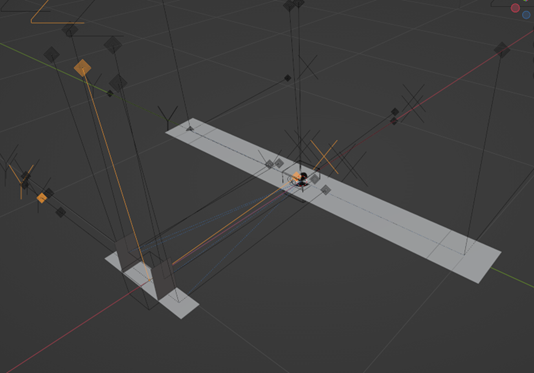
\includegraphics[width=0.9\linewidth]{Images/MBDyn model in blender.png}
    \caption{MBDyn model in Blender.}
    \label{fig:MBDyn_model_in_blender}
\end{figure}

\subsection{Reference System}
A reference system can be seen as a coordinate system used to describe the positions and orientations of elements. Because reference systems can be recursively built on each other, the process of building or transforming an MBDyn model is much easier when utilizing a reference system rather than building a model in the global system.

\subsection{Constitutive Law}
\label{section:Constitutive_law}
To realize the effect of ground contact, a Constitutive Law Module is applied in MBDyn, providing various formulas for 1D continuous contact models. This module can also function as a 3D constitutive law, under the assumption that the 1D formulas are applied with respect to the third direction of the associated 3D entity. In this case, the component three of strain and strain rate are utilized as inputs, and the output force is applied along direction three.

The Constitutive Law Module supports multiple models, including Flores, Hunt-Crossley, and Lankarani-Nikravesh. For this MBDyn model, the Flores model is used as the default. The dissipation coefficient (\(\text{dissipation\_coef}\)) is determined by the equation:

\begin{equation}
    \text{dissipation\_coef} = \frac{8}{5} \cdot \text{stiffness} \cdot \frac{1 - \text{restitution\_coef}}{\text{restitution\_coef} \cdot \dot{x}_0}
\end{equation}

It's important to note that the restitution coefficient (\(\text{restitution\_coef}\)) must satisfy \(0 < \text{restitution\_coef} \leq 1\). The stiffness parameter can be adjusted to approximate the behavior of the real ground. However, choosing an excessively high stiffness may cause the MBDyn simulation to stop abruptly if the drone experiences a hard impact with the ground. Therefore, a reasonable coefficient should be selected, balancing realism with stability.

A specific set of parameters for the constitutive law is chosen, as outlined in Table \ref{tab:Constitutive_law}.

\begin{table}[h]
    \centering
    \begin{tabular}{ccc}
    \hline
    Restitution Coefficient & Stiffness (\(\kappa\)) & Exponential Term \\
    \hline
    0.8 & \(2.4 \times 10^3\) & 1.5 \\
    \hline
    \end{tabular}
    \caption{Constitutive Law configuration}
    \label{tab:Constitutive_law}
\end{table}

To implement the constitutive law, 1 static node needs to be used to clamp on the ground, and 4 deformation displacement joints need to be used in 4 directions. A rigid free fall body from 1 meter height (figure \ref{fig:freefall}) is employed to evaluate the ground effect using the Constitutive Law Module.

\begin{figure}
    \centering
    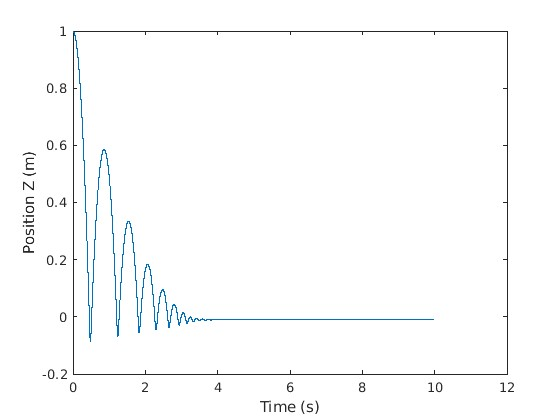
\includegraphics[width=0.5\linewidth]{Images/freefall.jpg}
    \caption{Position Change in Z-axis of free fall simulation.}
    \label{fig:freefall}
\end{figure}

\subsection{Data} 
The data module serves as the input mechanism, defining the geometry, physical properties, and initial conditions of the model.

\subsection{Initial Value} 
This module specifies the starting state of the model, including initial positions, velocities, and other parameters necessary for simulation initialization. The setup in the simulator is shown below.
\begin{itemize}
    \item Initial time: \(0\)
    \item Final time: \(100\)
    \item Time step: \(10^{-3}\)
    \item Tolerance: \(1 \times 10^{-10}\)
    \item Max iterations: \(10\)
    \item Derivatives tolerance: \(10\)
    \item Derivatives max iterations: \(200\)
    \item Derivatives coefficient: \(1 \times 10^{-3}\)
    \item Method: BDF
\end{itemize}

\subsection{Control Data} 
Control Data enables users to specify fundamental simulation parameters, including duration, time step size, and other global settings essential for the progression of the simulation process.

\textbf{Solver Configuration:} MBDyn offers a variety of solvers for simulating mechanical systems. Within the control data section, users can designate the preferred solver and configure its parameters, such as integration methods, convergence criteria, and tolerances.

\textbf{Output Configuration:} Users can define the desired output data, encompassing motion trajectories, forces, accelerations, and other pertinent information crucial for analysis and visualization purposes.

\textbf{Control Strategy:} Dynamic systems often require sophisticated control strategies to regulate system behavior over time. The control data section empowers users to define control algorithms, such as PID controllers or custom strategies, facilitating precise management of system dynamics during simulation.

\textbf{Error Handling and Logging:} MBDyn offers robust error handling and logging mechanisms during simulations. Users can specify error handling procedures and logging configurations to facilitate diagnosis and troubleshooting of simulation issues effectively.
\begin{verbatim}
begin: control data;
    structural nodes:
        +1      # CLAMP
        +1      # Mass Center
        +1      # ground
        +10     # dummy
    ;
    rigid bodies:
        1       # main body
    ;
    joints:
        +1      # ground clamp
        +1      # Mass Center
        +4      # constitutive law
    ;
    forces:
        20      # thrust and torque of propllers
    ;
    aerodynamic elements:
        +3      # Main
        +3      # H Tail
        +2      # V Tail
        +11     # aircraft intrument
    ;
    abstract nodes:
        +10     # angular velocity of motor
        +3      # Movable Surface
    ;
    genels:
        +10     # angular velocity delay function of motor
        +3      # Movable Surface
    ;
    gravity;
    air properties;
    output results : netcdf;
    output elements: 1;
    file drivers: 1;
    default orientation: euler321;
    default output: all;
end: control data;
\end{verbatim}

\subsection{Nodes} 
Nodes represent connection points or joints within the model, facilitating interactions between different components and defining the model's motion.

The type of nodes in MBDyn can be one of the following categories:
\begin{itemize}
    \item abstract
    \item electric
    \item hydraulic
    \item parameter
    \item structural
    \item thermal
\end{itemize}

\subsubsection{Structural Node}
Structural nodes can possess either six degrees of freedom (DOF), representing both position and orientation and thus describing the kinematics of rigid-body motion in space, or three degrees of freedom, representing position only and describing the kinematics of point mass motion in space.

The six-DOF structural node can be categorized as static, dynamic, modal, or dummy, while the three-DOF structural node can be either static or dynamic. Elements requiring only displacement can be connected to either type of node; however, when connected to a six-DOF node, they utilize solely position and velocity, contributing solely to force equilibrium equations. Elements necessitating both displacement and orientation are exclusive to six-DOF nodes.

\textbf{Static Node:} The static keyword means no inertia is related to that node, so it must be appropriately constrained or attached to elastic elements. Static nodes are useful when there is no need to apply inertia to them, thus saving 6 degrees of freedom. In this airframe, 1 static node (\textit{ClampNode}) is applied which is introduced in section \ref{section:Constitutive_law}.

\textbf{Dynamic Node:} The dynamic keyword means inertia can be attached to the node, so it provides linear and angular momenta degrees of freedom and automatically generates the so-called automatic structural elements. 2 Dynamic nodes (\textit{MassCenter}, \textit{ROOT}) need to be used, \textit{MassCenter} is a center to be acted on by aerodynamic force and propeller force and torque. \textit{MassCenter} and \textit{ROOT} are connected with 1 total joint to represent the force and torque which could be monitored in other software.

\textbf{Dummy Node:} The dummy structural node serves the purpose of facilitating the visualization of the kinematics of arbitrary points within the system during simulation. Unlike other structural nodes, the dummy node does not introduce any degrees of freedom itself; rather, it must be connected to another node within the system. This feature enhances the comprehensibility of the simulation output by allowing users to track the motion and behavior of specific points within the system. 10 dummy nodes are used in this airframe in each position of the propeller to apply the aircraft instruments which are introduced in section \ref{section:Aerodynamic elements}.

\subsubsection{Abstract Node}
Abstract nodes are ancestors of all scalar node types. Many general and electric elements can be connected to abstract nodes as well, since they directly use the ancestor class. 10 abstract nodes (\textit{ForceV1-8}, \textit{ForceH1}, \textit{ForceH2}) are used to apply the time delay and obtain the angular velocity of each propeller.

\subsection{Drivers} 
External forces or inputs applied to the model are defined by the drivers module, allowing users to simulate real-world effects and interactions.

\subsubsection{File Drives}
The \textit{Simulink} control system employs a WebSocket module to establish a connection with the MBDyn model. The input command comprises 12 inputs: the first three inputs control the surfaces for the aileron, elevator, and rudder respectively. Inputs 4 to 11 control the throttle for each vertical propeller, while 12 and 13 input controls the throttle for two horizontal propellers.

\subsection{Elements} 
Elements encompass the physical components or bodies within the model, defining their geometry, material properties, and connectivity.

\subsubsection{Rigid Body Element} 
The body element offers the possibility to add a point mass to a structural node. Additionally, inertia can be set.

In consideration of simulation accuracy and computation cost, the main structure in MBDyn is simplified to include only rigid bodies, due to the complex physical shape and negligible aerodynamic effect. The fuselage and the connecting components are neglected. To upgrade the structure of the airframe and provide the relevant information, including mass and inertia moment, the new values are as follows:

\begin{itemize}
    \item Mass: 6.4 kg
    \item Inertia Moment:
    \[
    \begin{pmatrix}
    0.3724 & 0.0004 & 0.0083 \\
    0.0004 & 0.7237 & 0 \\
    0.0083 & 0 & 1.0868 \\
    \end{pmatrix}
    \]
\end{itemize}

With these updated values, the airframe's mass and inertia moment are now accurately represented within the simulation environment. This enhanced structural representation ensures improved fidelity in the simulation results while balancing computational efficiency.

\subsubsection{Joint Element}
Since nodes must be constrained properly to satisfy the equilibrium equations in MBDyn, the joint element can be used to satisfy this request. Additionally, joints can be used to connect nodes together, relatively constraining certain degrees of freedom.

\textbf{Clamp Joint:} The clamp joint element constrains a node at all 6 degrees of freedom. Thus, this element can ideally be used to fix a base node, from which all other elements depend.

\textbf{Total Joint:} With the total joint element, constraints in each degree of freedom can be defined separately. Hereby MBDyn distinguishes between position and orientation constraints. Additionally, the constraints can be influenced in its value using a drive caller. Overall, this element can be used to arbitrarily define nodes' positions and motions.

\textbf{Deformable Displacement Joint:} This joint implements a configuration-dependent force that is exchanged between two points associated with two nodes with an offset. The force may depend, by way of a generic 3D constitutive law, on the relative position and velocity of the two points, expressed in the reference frame of node 1. The constitutive law is attached to the reference frame of node 1, so the sequence of the connections may matter in case of anisotropic constitutive laws if the relative orientation of the two nodes changes during the analysis.

\subsubsection{Force Element}
\label{section:force elements}
The force element has two types of forces that could be applied: structural and abstract. Structural forces have three components that may depend on arbitrary parameters (usually the simulated time) and a location in space. Structural couples have three parameter-dependent components.

Considering the difficulty and high computation cost of building each propeller with actual elements, currently, propeller parts are simplified as structural forces and torques applied at corresponding positions. The \textit{follower} in force and torque keeps the direction of force and moment fixed with the attitude of the main body of the airframe. The propulsion system consists of 8 propellers in the vertical direction, 4 of them are in front of the main wing, and another 4 vertical propellers are on the back of the main, and 2 horizontal propellers which are at the nose of the airframe. The actual positions are shown in Figure \ref{fig:Aircraft top view}.

\begin{figure}
    \centering
    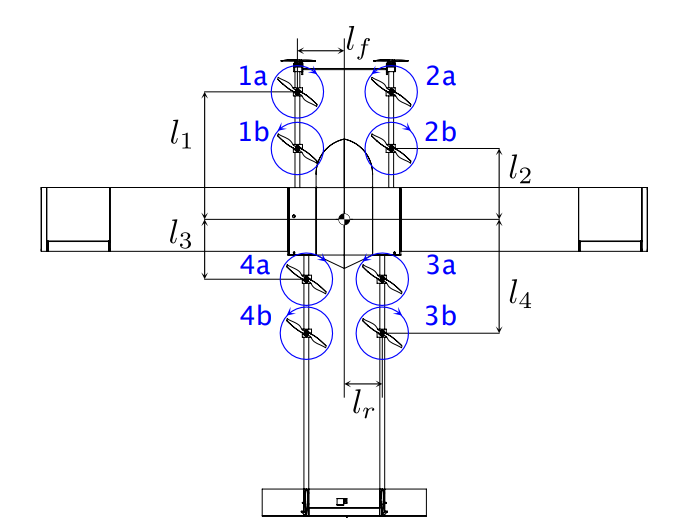
\includegraphics[width=0.8\linewidth]{Images/Aircraft top view.png}
    \caption{Aircraft top view, with relevant dimensions named, propellers numbering and propellers spinning directions.}
    \label{fig:Aircraft top view}
\end{figure}

The control system sends throttle command to rotor motors which drive vertical and horizontal propellers to achieve designed angular velocity to generate thrust and torque to provide the drone with lift and moments. The vertical propeller is controlled in multi-copter mode, and the horizontal propeller is controlled in fixed-wing mode. Considering the high computation cost of building each propeller with detailed aerodynamic bodies, the rotor is simplified as forces and moments at each rotor position.

In \cite{battaini2022}, Each of the propellers exerts a thrust and torque proportional to the square of the angular velocity:

\begin{equation}
    T_i = K_T \Omega_i^2,  K_T = C_T \rho A R^2, \label{eq:thrust} 
\end{equation}
\begin{equation}
    Q_i = K_Q \Omega_i^2,  K_Q = C_Q \rho A R^3, \label{eq:torque}
\end{equation}
where $C_T$ and $C_Q$ are the thrust and torque coefficients, $\rho$ is the air density, $A$ and $R$ are respectively the area of the propeller disk and its radius, and $\Omega_i$ is the rotational speed of the $i$-th propeller.

Previous work in \cite{battaini2022} simplified the propeller without considering the incoming flow, leading to high errors in real-world situations when the drone climbs, descends in multi-copter mode, or moves forward at high speed in fixed-wing mode. This section aims to optimize these equations. To consider the influence of inflow air, blade momentum theory and blade element theory need to be used.

\textbf{Blade Momentum Theory}

Blade Momentum Theory is a simplified method used to analyze the aerodynamic performance of rotor blades in rotary-wing aircraft such as helicopters \cite{Leishman2006}. It is based on the principle of conservation of momentum and assumes that the rotor extracts a constant amount of momentum from the air per unit time. The basic equation governing Blade Momentum Theory is:
\begin{equation}
    T = \dot{m} \cdot \Delta v \label{eq:Blade Momentum Theory}
\end{equation}
where:
\begin{itemize}
    \item $T$: Thrust produced by the rotor.
    \item $\dot{m}$: Mass flow rate of air through the rotor.
    \item $\Delta v$: Change in air velocity across the rotor.
\end{itemize}
The mass flow rate $\dot{m}$ is given by:
\begin{equation}
    \dot{m} = \rho \cdot A \cdot V
\end{equation}
where:
\begin{itemize}
    \item $\rho$: Air density.
    \item $A$: Rotor disk area.
    \item $V$: Airspeed.
\end{itemize}

\textbf{Blade Element Theory}

The blade element approach for the analysis of helicopter rotors has been well established \cite{Leishman2006}. The resultant local flow velocity at any blade element at a radial distance $y$ from the rotational axis has an out-of-plane component $U_P=V_c+v_i$ normal to the rotor as a result of climb and induced inflow and an in-plane component $U_T=\Omega y$ parallel to the rotor because of blade rotation, relative to the disk plane. The resultant velocity at the blade element is, therefore,
\begin{equation}
U=\sqrt{U_T^{2}+U_P^{2}}.
\end{equation}
The relative inflow angle (or induced angle of attack) at the blade element will be
\begin{equation}
\phi=\tan^{-1}\left(\frac{U_P}{U_T}\right)\approx\frac{U_P}{U_T} \text{ for small angles.}
\end{equation}
Thus, if the pitch angle at the blade element is $\theta$, then the aerodynamic or effective angle of attack is
\begin{equation}
\alpha=\theta-\phi=\theta-\frac{U_P}{U_T}.
\end{equation}
The resultant incremental lift $dL$ and drag $dD$ per unit span on this blade element are given by:
\begin{equation}
dL=\frac{1}{2}\rho U^{2}cC_l dy
\end{equation}
and
\begin{equation}
dD=\frac{1}{2}\rho U^{2}cC_d dy,
\end{equation}
where $C_l$ and $C_d$ are the lift and drag coefficients, respectively, and $c$ is the local blade chord.

\textbf{Thrust Approximation:} Based on steady linearized aerodynamics, the local blade lift coefficient can be written as
\begin{equation}
C_l = C_{l\alpha}(\alpha - \alpha_0) = C_{l\alpha}(\theta - \alpha_0 - \varphi),
\end{equation}
where $C_{l\alpha}$ is the 2-D lift-curve-slope of the airfoil section(s) comprising the rotor, and $\alpha_0$ is the corresponding zero-lift angle. For an incompressible flow, $C_{l\alpha}$ would have a value close to the thin-airfoil result of $2\pi$ per radian. Also, unless otherwise stated, it will be assumed that $\alpha_0$ can be combined into $\theta$.

Therefore, $C_{L_{w}}$ can be taken outside of the integral sign giving
\begin{equation}
    C_{T}=\frac{1}{2}\sigma\int_{0}^{1}C_{l}r^{2}dr=\frac{1}{2}\sigma~C_{l_{a}}\int_{0}^{1}(\theta-\phi)r^{2}dr,
\end{equation}
and using the result that $\phi=\lambda/r$ then the thrust coefficient can be written as
\begin{equation}
    C_{T}=\frac{1}{2}\sigma~C_{k}\int_{0}^{1}(\theta r^{2}-\lambda r)dr.
\end{equation}
In the condition of Untwisted Blades in Uniform Inflow, for a blade with zero twist, $\theta$ is constant ($\theta_0$), and for uniform inflow velocity, which is assumed in simple momentum theory, $\lambda$ is constant. Therefore, in this case, the thrust coefficient is given by
\begin{equation}
    C_{T}=\frac{1}{2}\sigma~C_{l_{*}}\int_{0}^{1}(\theta_{0}r^{2}-\lambda r)dr=\frac{1}{2}\sigma~C_{l_{*}}\left[\frac{\theta_{0}r^{3}}{3}-\frac{\lambda r^{2}}{2}\right]_{0}^{1}=\frac{1}{2}\sigma~C_{l_{a}}\left[\frac{\theta_{0}}{3}-\frac{\lambda}{2}\right]
\end{equation}

\textbf{Optimized derived Thrust and Torque of Rotor}

Based on these assumptions, (\ref{eq:Blade Momentum Theory}) from Blade Momentum Theory could be written as:
\begin{equation}
    T = 2 \rho A (v_c + u) u \label{eq:thrust_1}
\end{equation}
where:
\begin{itemize}
    \item $u$: outcome airflow.
    \item $v_c$: income airflow.
\end{itemize}
And in Blade Element Theory:
\begin{equation}
    \lambda = \frac{{(v_c + u)}}{{\omega R}}    \label{eq:thrust_2}
\end{equation}
\begin{equation}
    C_T = \frac{1}{2} \sigma C_{L\alpha} B^2 \left( \frac{{\theta B}}{3} - \lambda \right)  \label{eq:thrust_3}
\end{equation}
the thrust of the propeller could be written as:
\begin{equation}
    F = C_T \rho A \omega^2 R^2 \label{eq:thrust_4}
\end{equation}
Combining (\ref{eq:thrust_1}), (\ref{eq:thrust_2}), (\ref{eq:thrust_3}), and (\ref{eq:thrust_4}), the induced velocity in a generic cross-section is obtained:
\begin{equation}
    u = \sqrt{\frac{{B^4 C_{L\alpha}^2 \omega^2 R^2}}{{16}} + \frac{{4 \theta B^3 C_{L\alpha} \omega^2 R^2}}{3} - B^2 C_{L\alpha} \omega R v_c + 4 v_c^2} / 4 - \frac{{v_c}}{2} - \frac{{B^2 C_{L\alpha} \omega R}}{16}  \label{eq:outcome_airflow}
\end{equation}
(\ref{eq:outcome_airflow}) deviates the outcome airflow with the income airflow correction. Based on this, the corrected rotor thrust coefficient could be obtained by (\ref{eq:thrust_3}). For the torque generated by the propeller, in Torque-power approximations, according to blade element theory, by assuming uniform inflow and $C_d = C_{d0} = \text{constant}$, the torque coefficient with the inflow air correction could be obtained as:
\begin{equation}
    C_Q = \lambda C_T + \frac{1}{8} \sigma C_{d0}
\end{equation}
\cite{battaini2022} upgraded the motor and vertical propellers. After optimization, the new propellers used in the airframe are:

According to the propeller dimensions and experimental data provided in \cite{battaini2022}, the data used in the propeller is summarized in Table \ref{tab:propeller_specs}.

\begin{table}[h]
\centering
\caption{Propeller Coefficients}
\label{tab:propeller_specs}
\begin{tabular}{@{}lllllll@{}}
\hline
Propeller Type & Format & Dimension & $B$ & $\theta_0$ & $\sigma$ & $C_{D\alpha}$ \\
\hline
Horizontal & KDE 2304XF-2350 & 5x4.5 inch & 0.98 & $13^\circ$ & 0.187 & 0.26 \\
Vertical & KDE 2315XF-2050 & 7x4.2 inch & 0.98 & $17.3^\circ$ & 0.122 & 0.85 \\
\hline
\end{tabular}
\end{table}

\textbf{Comparison with MBDyn Rotor Model}

To prove the accuracy of derived thrust and torque equations, the previous thrust and moment equations applied in \cite{battaini2022} are also computed, and a detailed rotor aerodynamic MBDyn model is used as a reference to compare the thrust and torque in the same work condition. The data obtained in the previous section are used to build the MBDyn rotor model:

\begin{itemize}
    \item BLADE\_TWIST = 0
    \item INPUT\_THETA\_0
    \item OMEGA\_100 = 1917
    \item SIGMA
    \item R
    \item N\_B = 2
    \item N\_REVS = 20
\end{itemize}

A typical simulation result of the rotor MBDyn model is shown in Figure \ref{fig:aero_rotor Mbdyn}. After activation of the propeller at the initial phase, the force and moment of the rotor become stable values. The values of force and moment are chosen as the average value in the end phase.

As Figures \ref{fig:aero_rotor Thottle V} and \ref{fig:aero_rotor Thottle H} show, when propellers work without the influence of inflow wind, the force and moment in the optimized equation and MBDyn simulation are basically fit to the old simplified equation computed value. Because the MBDyn model could not build an absolute same model with the real propeller, the value of MBDyn simulation is a little different from the derived optimized equation and simplified equation.

In the simulation condition that constant 100\% throttle command with different inflow wind velocities (Figures \ref{fig:aero_rotor Wind H}, \ref{fig:aero_rotor Wind V}), it could be seen that the force and moment decrease with inflow velocity increase. Due to the MBDyn model accuracy, limitation of optimized equation that neglects the twist angle and tip loss effect, the difference between MBDyn simulation and estimate equation computed value increases with the increase of inflow velocity. Compared with other cases, the moment in the horizontal propeller has high error, but in actual simulation, the rotation orientation is opposite so that the moment value could be neglected. Basically, the optimized equation is enough to apply in actual MBDyn simulation.

The values are summarized in Tables \ref{tab:aero_rotor throttle H}, \ref{tab:aero_rotor throttle V}, and  \ref{tab:aero_rotor wind}.

\begin{figure}
    \centering
    \subfigure[Force]{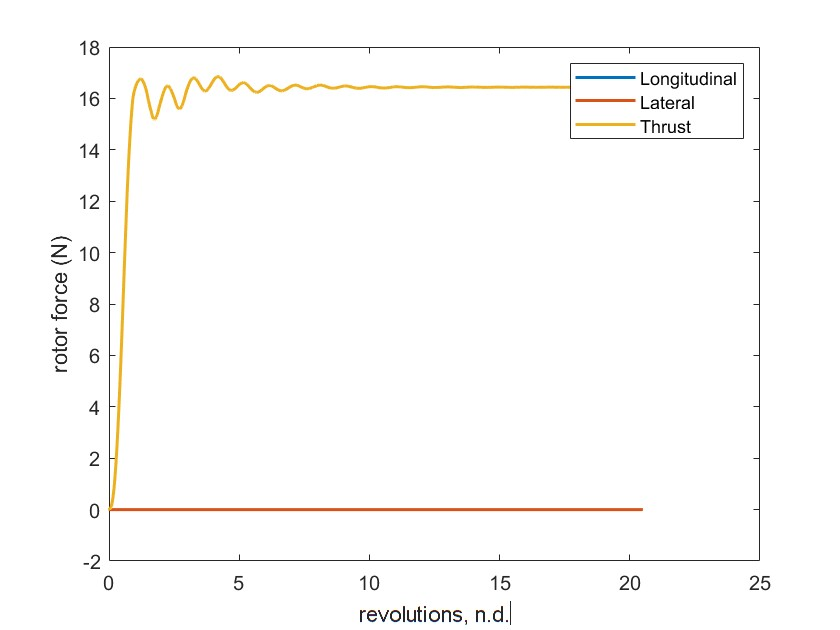
\includegraphics[width=0.3\textwidth]{Images/aero_rotor/aerorotor force_V0.jpg}}
    \hfil % Add some horizontal space between the figures
    \subfigure[Moment]{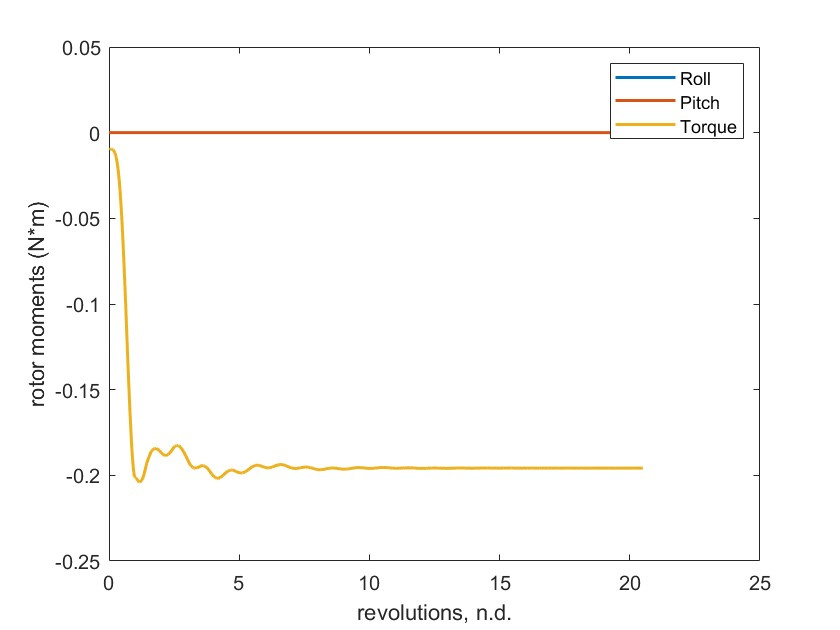
\includegraphics[width=0.3\textwidth]{Images/aero_rotor/aerorotor moment_V0.jpg}}    
    \hfil % Add some horizontal space between the figures
    \subfigure[Induced Velocity]{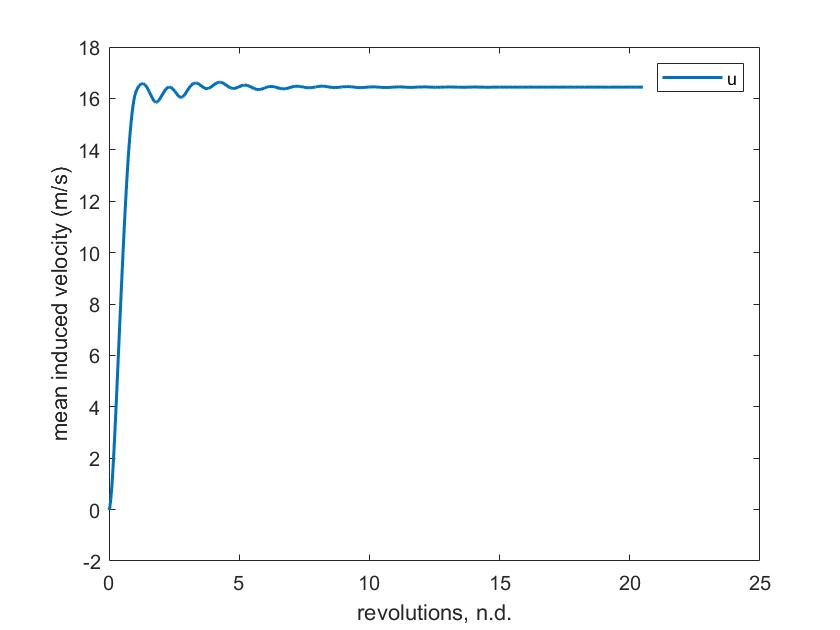
\includegraphics[width=0.3\textwidth]{Images/aero_rotor/aerorotor Velocity_V0.jpg}}    
    \caption{Force and moment change of rotor MBDyn simulation}
    \label{fig:aero_rotor Mbdyn}
\end{figure}

\begin{figure}
    \centering
    \subfigure[Force]{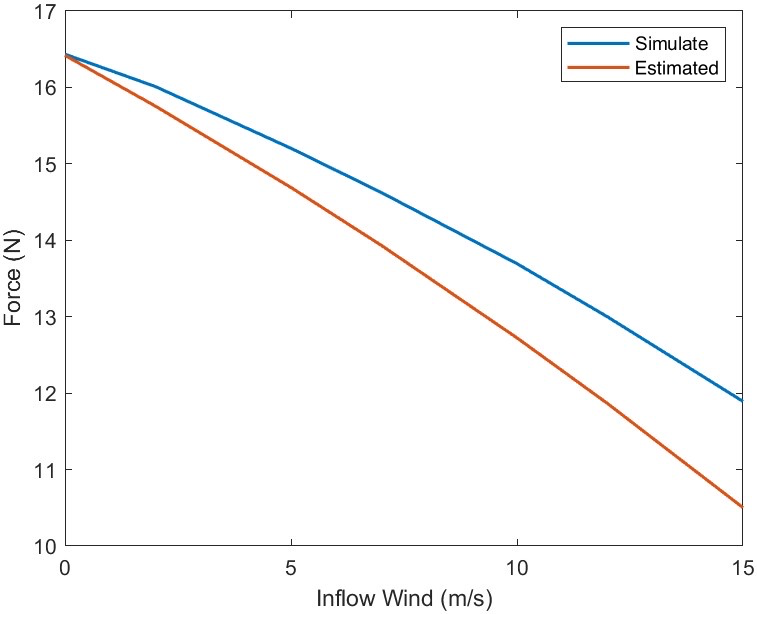
\includegraphics[width=0.4\textwidth]{Images/aero_rotor/aerorotor Force V Wind.png}}
    \hfil % Add some horizontal space between the figures
    \subfigure[Moment]{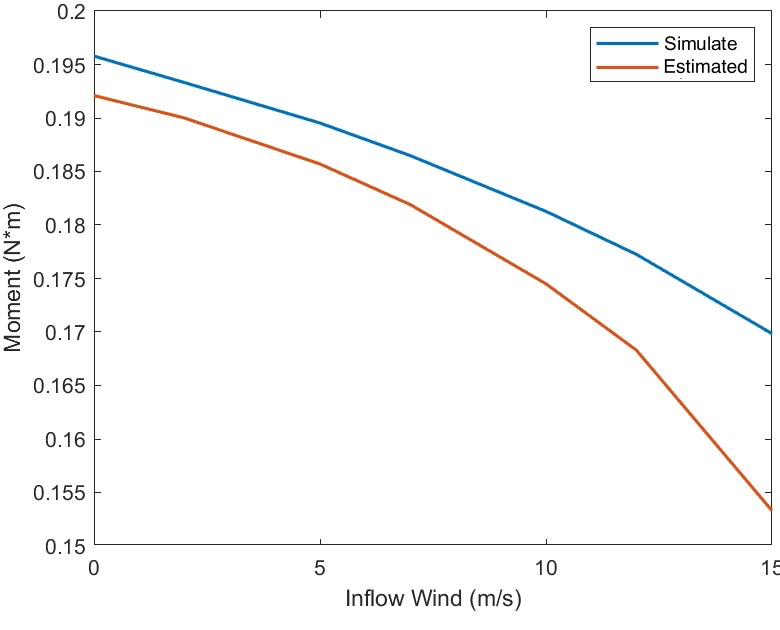
\includegraphics[width=0.4\textwidth]{Images/aero_rotor/aerorotor Moment V Wind.png}}
    \caption{Comparison between optimized equation computed value and MBDyn simulation with change of inflow velocity in vertical propellers.}
    \label{fig:aero_rotor Wind V}
\end{figure}

\begin{figure}
    \centering
    \subfigure[Force]{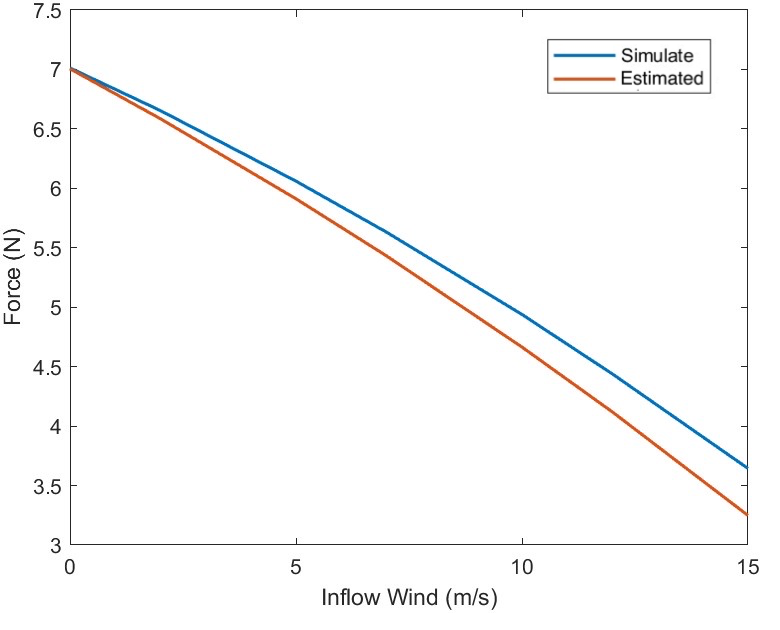
\includegraphics[width=0.4\textwidth]{Images/aero_rotor/aerorotor Force H Wind.png}}
    \hfil % Add some horizontal space between the figures
    \subfigure[Moment]{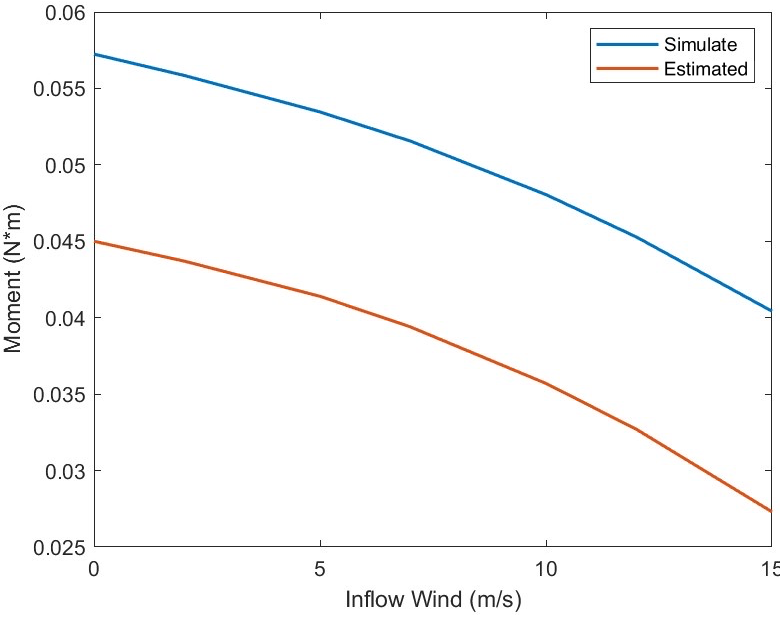
\includegraphics[width=0.4\textwidth]{Images/aero_rotor/aerorotor Moment H Wind.png}} 
    \caption{Comparison between optimized equation computed value and MBDyn simulation with change of inflow velocity in horizontal propellers.}
    \label{fig:aero_rotor Wind H}
\end{figure}

\begin{figure}
    \centering
    \subfigure[Force]{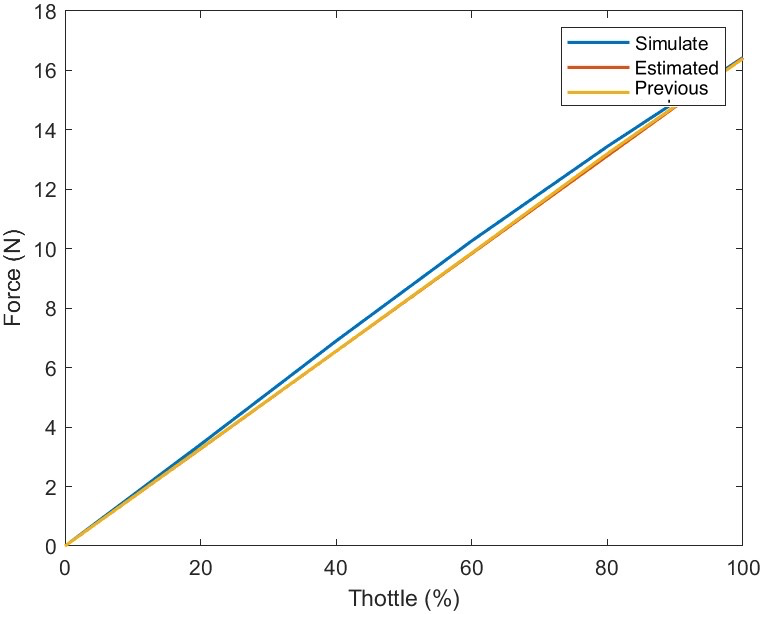
\includegraphics[width=0.4\textwidth]{Images/aero_rotor/aerorotor Force V Thottle.png}}
    \hfil % Add some horizontal space between the figures
    \subfigure[Moment]{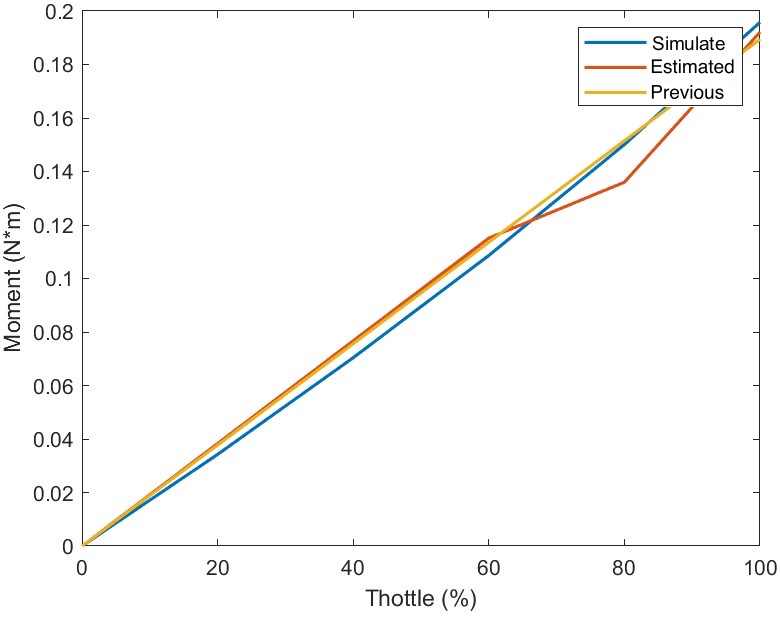
\includegraphics[width=0.4\textwidth]{Images/aero_rotor/aerorotor Moment V Thottle.png}}    
    \caption{Change with Thottle}
    \label{fig:aero_rotor Thottle V}
\end{figure}

\begin{figure}
    \centering
    \subfigure[Force]{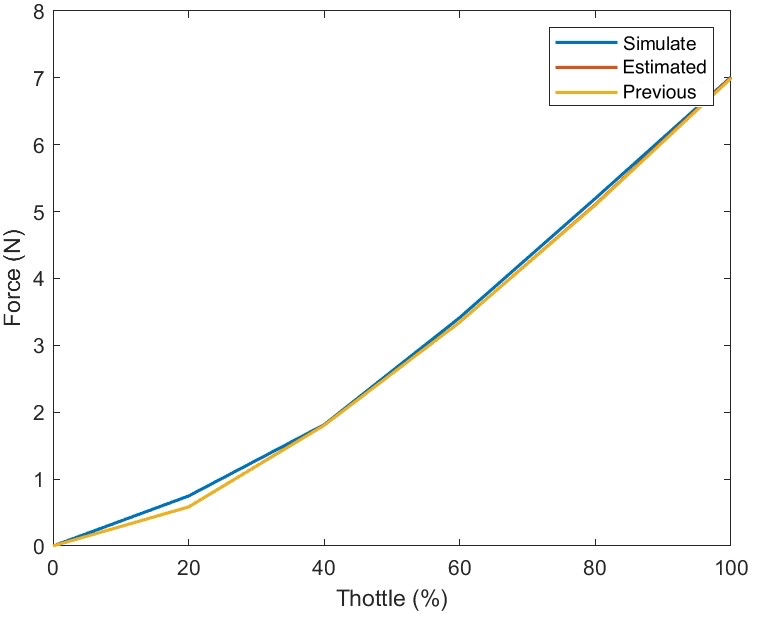
\includegraphics[width=0.4\textwidth]{Images/aero_rotor/aerorotor Force H Thottle.png}}
    \hfil % Add some horizontal space between the figures
    \subfigure[Moment]{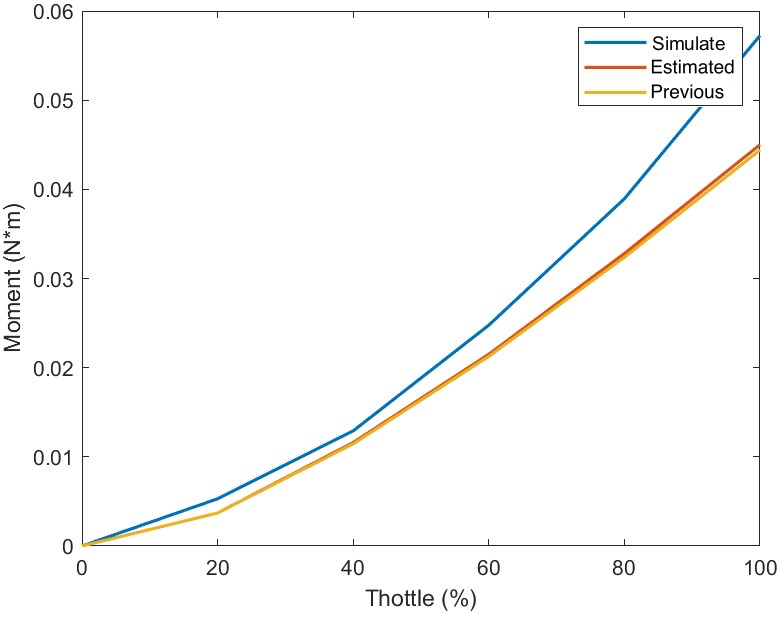
\includegraphics[width=0.4\textwidth]{Images/aero_rotor/aerorotor Moment H Thottle.png}}    
    \caption{Comparison between optimized equation computed value, MBDyn simulation and old simplified equation computed value with change of throttle command.}
    \label{fig:aero_rotor Thottle H}
\end{figure}

\begin{sidewaystable}
\centering
\caption{Comparison between optimized equation computed value and MBDyn simulation with change of inflow velocity in vertical and horizontal propellers.}
\begin{tabular}{c|cc|cc|cc|cc}
\hline
Inflow Velocity (m/s) & \multicolumn{4}{c}{Vertical propeller} & \multicolumn{4}{c}{Horizontal propeller} \\
\hline
       & \multicolumn{2}{c}{Force (N)}  & \multicolumn{2}{c}{Moment (N*m)} & \multicolumn{2}{c}{Force (N)}  & \multicolumn{2}{c}{Moment (N*m)}\\
       \hline
       & Simulation & Estimated & Simulation & Estimated & Simulation & Estimated & Simulation & Estimated \\
       \hline
0      & 16.4345 & 16.4191 & 0.195786 & 0.1921 & 7.01236 & 7.0054 & 0.0572453 & 0.045 \\
2      & 16.0111 & 15.7553 & 0.193313 & 0.19   & 6.65378 & 6.5854 & 0.0558456 & 0.0437 \\
5      & 15.2033 & 14.6906 & 0.189529 & 0.1857 & 6.06021 & 5.9119 & 0.0534594 & 0.0414 \\
7      & 14.6242 & 13.9332 & 0.186478 & 0.1819 & 5.6318  & 5.4323 & 0.0515545 & 0.0394 \\
10     & 13.6939 & 12.7228 & 0.18127  & 0.1745 & 4.93898 & 4.6645 & 0.0480527 & 0.0357 \\
12     & 12.9989 & 11.8653 & 0.177255 & 0.1683 & 4.43862 & 4.1191 & 0.0452798 & 0.0327 \\
15     & 11.8917 & 10.5018 & 0.169847 & 0.1533 & 3.64383 & 3.2484 & 0.0404258 & 0.0273 \\
\hline
\label{tab:aero_rotor wind}
\end{tabular}
\end{sidewaystable}

\begin{table}[htbp]
\centering
\caption{Comparison between optimized equation computed value, MBDyn simulation and old simplified equation computed value in vertical propeller with change of throttle command.}

\begin{tabular}{c|ccc|ccc}
\hline
Throttle(\%) & \multicolumn{3}{c}{Force(N)} & \multicolumn{3}{c}{Moment(N*m)} \\
\hline
 & Simulation & Estimated & Previous & Simulation & Estimated & Previous  \\
 \hline
0   & 0        & 0        & 0        & 0         & 0        & 0         \\
20  & 3.41705  & 3.2702   & 3.275202 & 0.0342378 & 0.0383   & 0.037727  \\
40  & 6.89989  & 6.5544   & 6.564398 & 0.0703868 & 0.0767   & 0.075615  \\
60  & 10.267   & 9.8419   & 9.856905 & 0.108608  & 0.1151   & 0.113541  \\
80  & 13.4427  & 13.1302  & 13.150217& 0.150066  & 0.136    & 0.151476  \\
100 & 16.4345  & 16.4191  & 16.444145& 0.195786  & 0.1921   & 0.189418  \\
\hline
\label{tab:aero_rotor throttle V}
\end{tabular}
\end{table}

\begin{table}[htbp]
\centering
\caption{Comparison between optimized equation computed value, MBDyn simulation and old simplified equation computed value in horizontal propeller with change of throttle command.}
\begin{tabular}{c|ccc|ccc}
\hline
Throttle (\%) & \multicolumn{3}{c}{Force (N)} & \multicolumn{3}{c}{Moment (N*m)} \\
\hline
 & Simulation & Estimated & Previous & Simulation & Estimated & Previous \\
 \hline
0   & 0        & 0        & 0        & 0         & 0        & 0         \\
20  & 0.747664 & 0.5837   & 0.582698 & 0.005292  & 0.0037   & 0.003700  \\
40  & 1.81467  & 1.8073   & 1.804101 & 0.012908  & 0.0116   & 0.011456  \\
60  & 3.41634  & 3.3472   & 3.349052 & 0.024764  & 0.0215   & 0.021267  \\
80  & 5.19855  & 5.1078   & 5.098734 & 0.038943  & 0.0328   & 0.032378  \\
100 & 7.01236  & 7.0054   & 6.992987 & 0.057245  & 0.045    & 0.044406  \\
\hline
\label{tab:aero_rotor throttle H}
\end{tabular}
\end{table}

In the MBDyn model, the thrust and torque are applied by force and couple elements, using string type to compute the value of the equations. A dummy node provides income airflow in corresponding rotor positions. The angular velocity value of each propeller is obtained from the Simulink throttle command after processing in genel elements.

\subsubsection{Aerodynamic Elements}
\label{section:Aerodynamic elements}

To build the main wings and tail wings structure, aerodynamic elements should be applied to construct wings as rigid wings, as this model primarily focuses on the lift and drag forces acting on the airframe. Air properties are added to simulate the necessary environmental conditions about air. Aircraft instruments are used to monitor aircraft status information.

\textbf{Air Properties}

In MBDyn, airstream properties are determined by the air's physical attributes and the velocity's direction and magnitude. Standard SI units are employed, with adjustments made for a temperature deviation of -55 K and a reference altitude of 1000 m. Users can also provide parameters for computing air properties based on the requested z-position. These parameters include reference pressure $p_0$, reference density $\rho_0$, reference temperature $T_0$, initial temperature gradient $\frac{dT}{dz}$, gas constant $R$, initial gravity acceleration $g_0$, and the bottom and top altitudes of the null temperature gradient region $z_1$ and $z_2$. In this model, the temperature deviation and reference altitude are set to zero.

\textbf{Gust Wind:} Using the optional \texttt{gust} keyword enables the incorporation of a gust model. A basic gust model represents a uniform change in airstream speed and direction, achieved through a time-dependent airstream drive. To simulate the drone's performance in gusty conditions, gust wind is applied in different simulation scenarios. The Front 1D Gust model is chosen to simulate wind passing through the drone, providing a uniform front:
\[
\mathbf{v}(x, t) = n g(V_{\text{ref}} \cdot t - f \cdot x)
\]
where:
\begin{itemize}
    \item $\mathbf{v}$ is the velocity perturbation in the global frame.
    \item $x$ is the position, in the global frame, of the point whose airstream velocity is being evaluated.
    \item $t$ is the current time.
    \item $n$ is the unit vector perturbation\_direction that defines the direction of the velocity perturbation in the global frame.
    \item $g(\cdot)$ is the function front\_profile that defines the gust profile as a function of $x = V_{\text{ref}} \cdot t - f \cdot x$, i.e., the local position (in units of length) of the measure point in a frame moving with the gust front along the $f$ direction.
    \item $f$ is the unit vector front\_direction that defines the direction of propagation of the front in the global frame.
    \item $V_{\text{ref}}$ is the constant velocity front\_velocity of propagation of the front in direction $f$.
\end{itemize}

The wind curve chooses cosine signal as a curve to simulate the real gust environment. Typical gusts move along the X, Y, Z-axis, which need to be considered separately in multi-copter control mode and fixed-wing control mode.

\textbf{Aerodynamic Body}

The elements differ in their treatment of aerodynamics: one assumes a rigid surface from a single node.

The \texttt{control\_drive} parameter, combined with angle of attack, simulates control surface deflection across the element. It's calculated using the ratio of lift stability to control derivatives.

\begin{equation}
    \text{Control\_Drive} = \frac{C_{L/\delta}} {C_{L/\alpha}} \delta
\end{equation}

Aircraft motion through air generates aerodynamic forces and moments, crucial for flight prediction. These depend on surface interaction, geometry, angle of attack, and airspeed.

\textbf{Equations of Motion}

The equations of motion for an aircraft can be expressed as follows:

\begin{align}
    \sum F_x &= m \cdot a_x \\
    \sum F_y &= m \cdot a_y \\
    \sum F_z &= m \cdot a_z \\
    \sum M_x &= I_x \cdot \alpha_x \\
    \sum M_y &= I_y \cdot \alpha_y \\
    \sum M_z &= I_z \cdot \alpha_z
\end{align}

where:
\begin{itemize}
    \item $F_x$, $F_y$, $F_z$: Forces in the $x$, $y$, and $z$ directions, respectively.
    \item $M_x$, $M_y$, $M_z$: Moments about the $x$, $y$, and $z$ axes, respectively.
    \item $m$: Mass of the aircraft.
    \item $a_x$, $a_y$, $a_z$: Accelerations in the $x$, $y$, and $z$ directions, respectively.
    \item $I_x$, $I_y$, $I_z$: Moments of inertia about the $x$, $y$, and $z$ axes, respectively.
    \item $\alpha_x$, $\alpha_y$, $\alpha_z$: Angular accelerations about the $x$, $y$, and $z$ axes, respectively.
\end{itemize}

\textbf{Aerodynamic Coefficients}

The aerodynamic forces and moments can be expressed in terms of aerodynamic coefficients, which are dimensionless parameters that depend on the geometry of the aircraft and its flight conditions. Some commonly used aerodynamic coefficients include:

\begin{itemize}
    \item Lift coefficient ($C_L$)
    \item Drag coefficient ($C_D$)
    \item Side force coefficient ($C_Y$)
    \item Roll moment coefficient ($C_l$)
    \item Pitch moment coefficient ($C_m$)
    \item Yaw moment coefficient ($C_n$)
\end{itemize}

These coefficients can be related to the aerodynamic forces and moments using the following equations:

\begin{align}
    L &= \frac{1}{2} \rho V^2 S C_L \\
    D &= \frac{1}{2} \rho V^2 S C_D \\
    Y &= \frac{1}{2} \rho V^2 S C_Y \\
    L &= \frac{1}{2} \rho V^2 S C_l \\
    M &= \frac{1}{2} \rho V^2 S C_m \\
    N &= \frac{1}{2} \rho V^2 S C_n
\end{align}

where:
\begin{itemize}
    \item $L$, $D$, $Y$: Lift, drag, and side force, respectively.
    \item $M$, $N$: Pitch and yaw moments, respectively.
    \item $\rho$: Air density.
    \item $V$: Airspeed.
    \item $S$: Reference area of the aircraft.
\end{itemize}

These equations provide a framework for understanding the aerodynamic forces and moments acting on an aircraft and are essential for aircraft design, analysis, and control.

\textbf{Wing}

Based on the previous work in \cite{battaini2022}, the wing part could be modeled in the main wing and tail wing with 1 horizontal tail wing and 2 vertical tail wings. According to the information from \cite{martello2021} and \cite{battaini2022}, the main wing section of the drone utilizes the Selig 2046 airfoil, while other airfoil sections employ the NACA 0008 airfoil. In the MBDyn software, lift coefficient, drag coefficient, and moment coefficient for a specific airfoil are interpolated by C81 format file, which is obtained from \cite{airfoiltools}.
the detailed data \cite{airfoiltools} are shown in Table \ref{tab:aero_coeffs}. Due to the lack of aerodynamic coefficient in high angle of attack, this part is replaced with default data of NACA 0012 provided by MBDyn.

\begin{figure}
    \centering
    \subfigure[Curve of $C_l$ and $C_d$ aerodynamic coefficient]{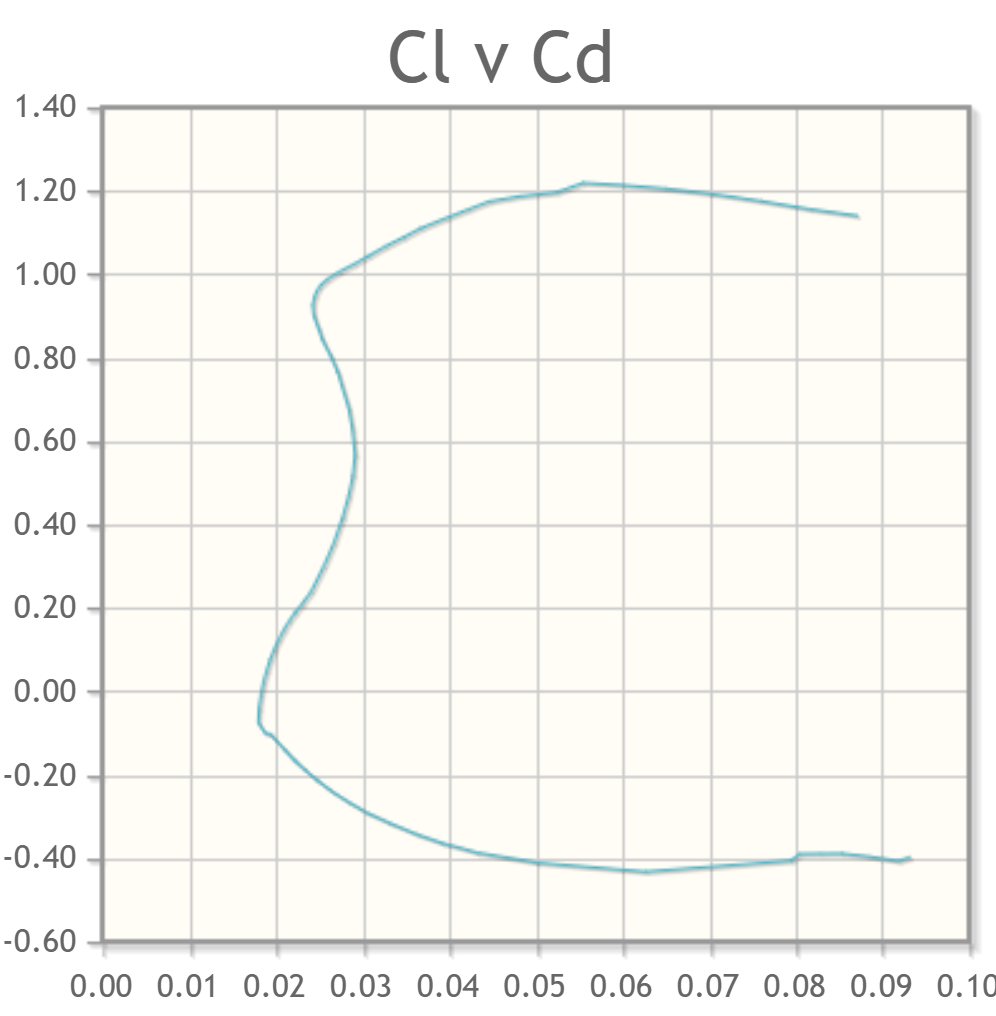
\includegraphics[width=0.4\textwidth]{Images/s2046 clvcd.png}}
    \hfil % Add some horizontal space between the figures
    \subfigure[Curve of $C_l$ and angle of attack]{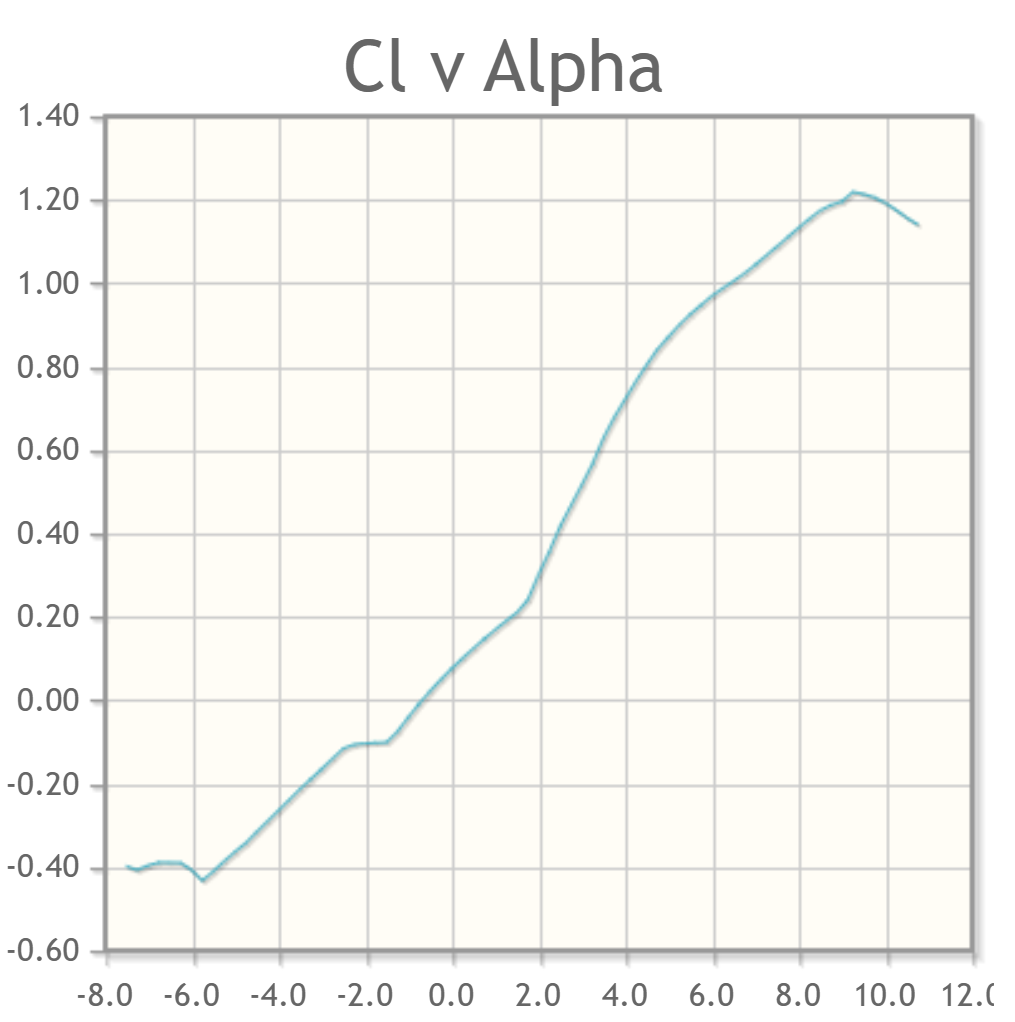
\includegraphics[width=0.4\textwidth]{Images/s2046 clvalpha.png}}    
    \caption{Selig 2046 airfoil aerodynamic coefficient Curve}
    \label{fig:aerodynamic coefficient Selig 2046}
\end{figure}

\begin{figure}
    \centering
    \subfigure[Curve of $C_l$ and $C_d$ aerodynamic coefficient]{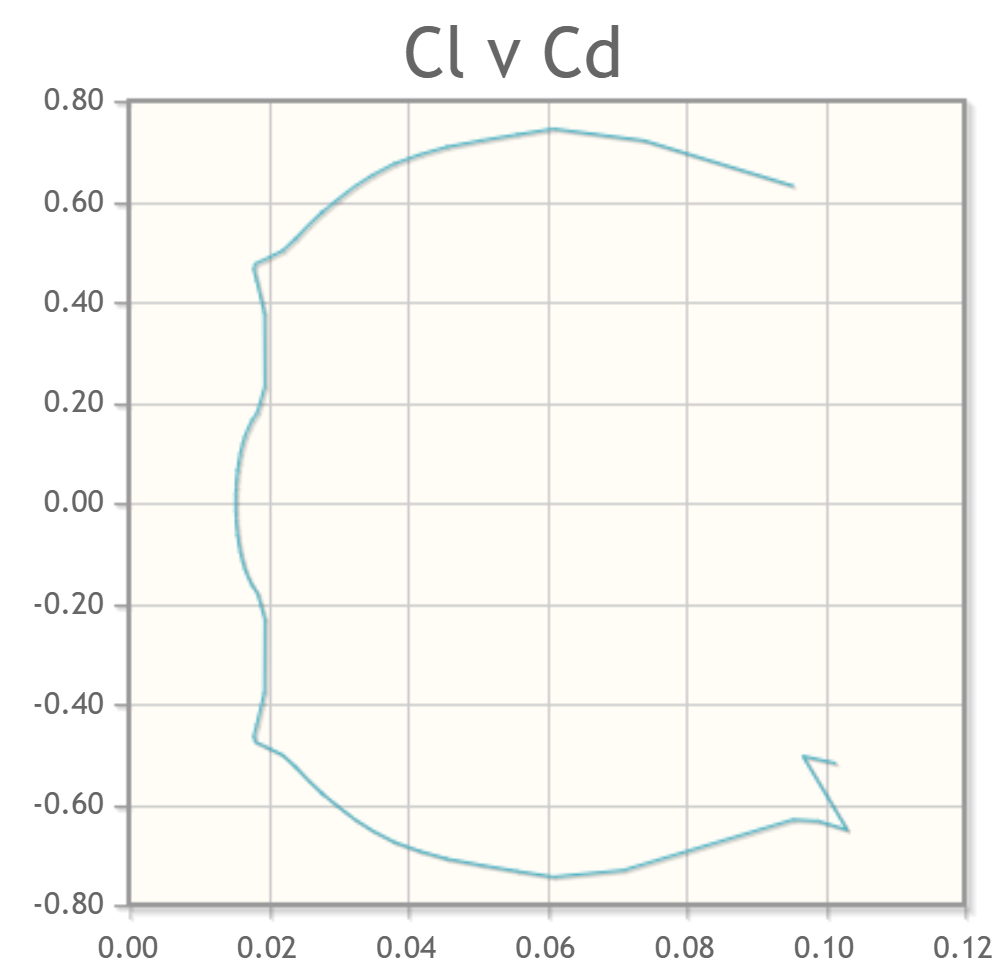
\includegraphics[width=0.4\textwidth]{Images/naca008 clvcd.png}}
    \hfil % Add some horizontal space between the figures
    \subfigure[Curve of $C_l$ and angle of attack]{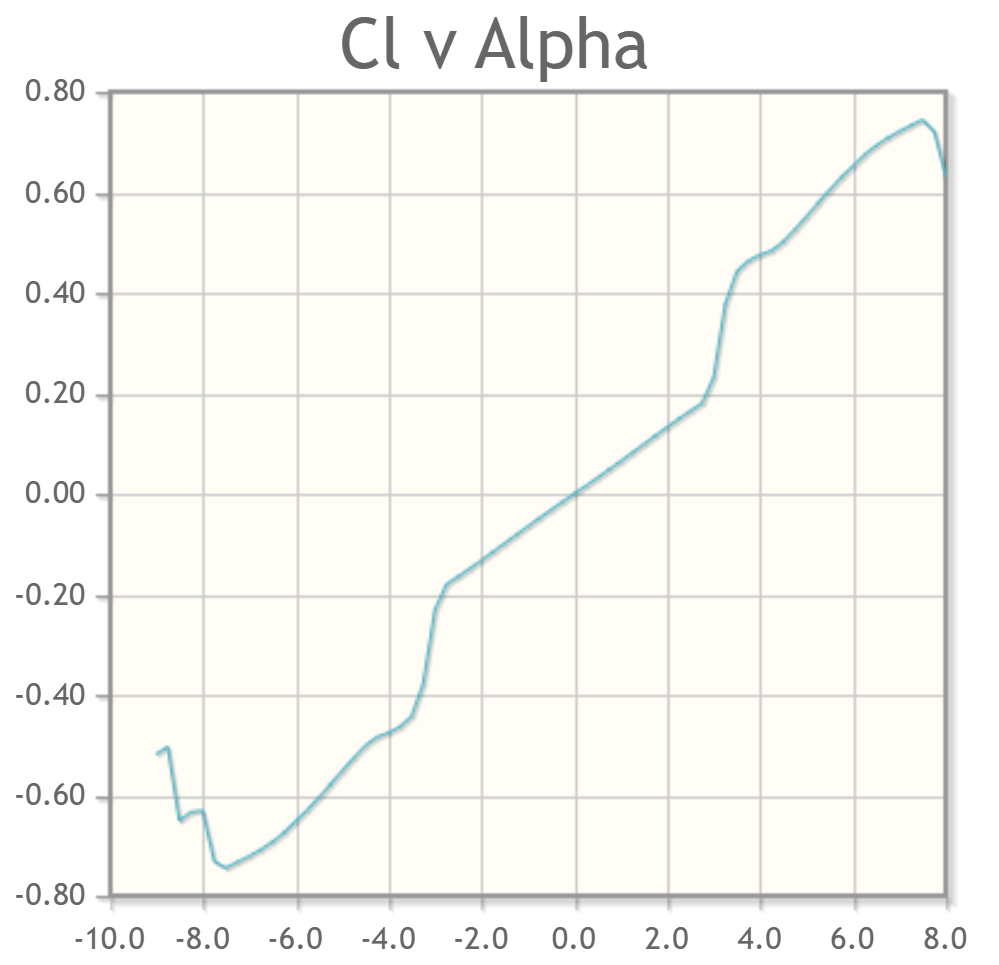
\includegraphics[width=0.4\textwidth]{Images/naca008 clvalpha.png}}    
    \caption{NACA 0008 airfoil aerodynamic coefficient Curve}
    \label{fig:aerodynamic coefficient naca 0008}
\end{figure}

\begin{table}[h]
\centering
\caption{C81 Data for Selig 2046 and NACA0008 Airfoils}
\label{tab:aero_coeffs}
\begin{tabular}{|c|c|c|c|c|c|c|}
\hline
\multirow{2}{*}{$\alpha$ (deg)} & \multicolumn{3}{c|}{S2046} & \multicolumn{3}{c|}{NACA0008} \\
\cline{2-7}
 & $C_{l\alpha}$ & $C_{d\alpha}$ & $C_{m\alpha}$ & $C_{l\alpha}$ & $C_{d\alpha}$ & $C_{m\alpha}$ \\
\hline
-2.50 & -0.1157 & 0.02003 & -0.0574 & -0.1649 & 0.01782 & -0.0122 \\
-2.25 & -0.1059 & 0.01961 & -0.0518 & -0.1490 & 0.01724 & -0.0119 \\
-2.00 & -0.1033 & 0.01962 & -0.0448 & -0.1325 & 0.01677 & -0.0112 \\
-1.75 & -0.1017 & 0.01941 & -0.0381 & -0.1157 & 0.01641 & -0.0104 \\
-1.50 & -0.1007 & 0.01888 & -0.0317 & -0.0988 & 0.01611 & -0.0093 \\
-1.25 & -0.0752 & 0.01807 & -0.0311 & -0.0818 & 0.01588 & -0.0081 \\
-1.00 & -0.0408 & 0.01816 & -0.0349 & -0.0649 & 0.01571 & -0.0067 \\
-0.75 & -0.0085 & 0.01838 & -0.0378 & -0.0483 & 0.01557 & -0.0052 \\
-0.50 & 0.0215 & 0.01867 & -0.0399 & -0.0319 & 0.01548 & -0.0035 \\
-0.25 & 0.0494 & 0.01903 & -0.0416 & -0.0158 & 0.01543 & -0.0018 \\
0.00 & 0.0757 & 0.01944 & -0.0428 & 0.0000 & 0.01541 & 0.0000 \\
0.25 & 0.1005 & 0.01991 & -0.0437 & 0.0158 & 0.01543 & 0.0018 \\
0.50 & 0.1243 & 0.02043 & -0.0445 & 0.0319 & 0.01548 & 0.0035 \\
0.75 & 0.1470 & 0.02100 & -0.0451 & 0.0483 & 0.01557 & 0.0052 \\
1.00 & 0.1689 & 0.02164 & -0.0456 & 0.0649 & 0.01570 & 0.0067 \\
1.25 & 0.1898 & 0.02235 & -0.0461 & 0.0818 & 0.01588 & 0.0081 \\
1.50 & 0.2099 & 0.02313 & -0.0465 & 0.0988 & 0.01611 & 0.0093 \\
1.75 & 0.2396 & 0.02418 & -0.0489 & 0.1158 & 0.01640 & 0.0104 \\
2.00 & 0.3003 & 0.02563 & -0.0566 & 0.1326 & 0.01677 & 0.0112 \\
2.25 & 0.3561 & 0.02679 & -0.0630 & 0.1490 & 0.01724 & 0.0119 \\
2.50 & 0.4167 & 0.02779 & -0.0696 & 0.1649 & 0.01782 & 0.0122 \\
\hline
\end{tabular}
\end{table}

Consider the implementation of control movable surfaces on the wings. For each wing, the main wings and horizontal tail wing need to be modeled separately.

\textbf{Main Wings:}
\begin{itemize}
    \item 3 elements
    \item Mid fixed wing, left and right wing with airfoil
    \item Each wing includes aileron control surfaces
    \item The aileron part constitutes 20\% of the modeled aerodynamic wing surface
    \item Considering the presence of the tip part, the actual ratio $\beta$ is 0.19
\end{itemize}

For the horizontal tail wing, which has an elevator control surface at the center of the aerodynamic wing surface, the horizontal surface is separated into 3 elements.

\textbf{Tail Wings:}
\begin{itemize}
    \item 5 elements
    \item Mid horizontal tail wing with elevator
    \item Left and right horizontal fixed tail wing
    \item 2 vertical tail wings with rudder
    \item The ratio $\beta$ is 30\% for both the horizontal and vertical tail wings
    \item Considering the presence of the tip part, the actual value of $\beta$ is 0.25
\end{itemize}

\begin{align}
    \beta_{\text{aileron}} = 0.1764 \\
    \beta_{\text{elevator}} = 0.3 \\
    \beta_{\text{rudder}} = 0.1050
\end{align}

\textbf{Aircraft Instruments}

The \texttt{aircraft\_node} in MBDyn represents the aircraft within a defined reference frame. By default, the positive x-direction aligns with the tail-to-nose axis, the positive z-direction aligns with the top-to-bottom axis, and the positive y-direction aligns with the rightward direction relative to the pilot. An optional orientation parameter can be specified for adjustments.

During simulation, various measures related to the aircraft's dynamics are accessible, such as airspeed, altitude, attitude, turn rate, and more. Additional data, like initial position, accelerations, and environmental conditions, are also available.

These parameters provide essential data for analyzing the aircraft's behavior and performance within the simulation environment.

\textbf{Body Velocity of Propeller:} In the part of force and moment element for the propeller, the airspeed of each propeller in the thrust direction is necessary to be used as the correction factor to generate the force and moment for each propeller. Considering the rotational movement of the drone itself and the influence of gust wings on the airspeed in complex test environments, using only the status data in the \textit{MassCenter} node is not accurate enough. A dummy node could be applied as sub-nodes for dynamic nodes, which could be used to build separate aircraft instruments in the position of every propeller. Use aircraft instruments to get the airspeed in the X-axis in the body frame of the drone for horizontal propellers and the airspeed in the Z-axis in the body frame of the drone for vertical propellers.

In addition to the aircraft instrument used for the propeller, another aircraft instrument is needed to be applied in the \textit{MassCenter} to monitor status information, such as airspeed, attitude angle, angular velocity, angular acceleration, etc. These data would be output by the output element part.

\subsubsection{General Elements}

To implement hardware delay in MBDyn, a scalar filter as a transfer function within General Elements is crucial.

This element models a scalar filter with the equation:
\begin{equation}
    A(s) y = B(s) u
\end{equation}
where \( A \) and \( B \) are polynomials of arbitrary order:
\begin{equation}
    y(s) = \frac{{b_0 s^{n_n} + b_1 s^{n_n-1} + \ldots + b_{n_n}}}{{a_0 s^{n_d} + a_1 s^{n_d-1} + \ldots + a_{n_d}}}u(s) 
\end{equation}
The filter must be proper, meaning \( n_d \) (output order) must be greater than or equal to \( n_n \) (input order). Polynomial \( A \) is monic (\( a_0 = 1 \)), and only coefficients from \( a_1 \) to \( a_n \) are needed. All coefficients of polynomial \( B \) must be provided, from \( b_0 \) to \( b_{n_n} \).

If a gain is supplied, all coefficients of \( B \) are multiplied by the gain.

Originally, input was required from a ScalarDof; now, it can also be taken from a drive, simplifying setup complexity.

In actual control situations, there is a hardware delay time that should be considered. In \cite{martello2021}, the actual delay time for movable surfaces has been provided. Referring to the data provided in \cite{battaini2020} on the Corona 939 Metal Gear servomotor \cite{CoronaServo} used for controlling surfaces, a time delay of 0.13 seconds is reported for movable surface control.

In \cite{battaini2022}, the actual delay time for the propeller has been provided. According to the experimental results in \cite{martello2021}, the delay time range is between 0.19 seconds and 0.27 seconds. For the MBDyn model, 0.25 seconds is chosen as the delay time applied in MBDyn.

These time delays for vertical propellers, horizontal propellers, and control surface actuation, as mentioned above, are integrated into the model using abstract nodes. The time delay for vertical propellers, which is upgraded in \cite{battaini2022}, is 0.015 seconds, and the time delay for horizontal propellers, which is designed in \cite{martello2021}, is 0.25 seconds.

Differential of Abstract Node and Scalar filter of Genel element is used to realize the delay effect in MBDyn. The transfer function is shown below:
\begin{equation}
    H(s) = \frac{\frac{1}{\tau}}{s+\frac{1}{\tau}}
\end{equation}
where \( \tau \) is a constant time value, set as the time delay value for each element.

Because the input command is the throttle of the motor, which needs to be computed to the actual angular velocity of the propeller used in the thrust or moment computation. The quadratic model between the angular velocity of the propeller and throttle command could be described as:
\begin{equation}
    th = a \cdot \Omega^2 + b \cdot \Omega \label{eq:th2Omega}
\end{equation}
where: \\
\(th\) is throttle command from the control system in percentage\\
\(\Omega\) is achieved angular velocity of the propeller
By equation (\ref{eq:th2Omega}), the relationship between angular velocity \( \Omega \) and throttle command \( th \) could be derived as:
\begin{equation}
    \Omega = \frac{- b + \sqrt{ b ^ 2 + 4 \cdot a \cdot th }}{2 \cdot a}
\end{equation}
The coefficients \( a \) and \( b \) of the vertical propeller, obtained with least square fitting in \cite{battaini2022}. To keep same in horizontal propeller, the coefficients \( a \) and \( b \) of horizontal propellers are also fitted using square fitting, are summarized in Table \ref{tab:Angular velocity against throttle quadratic model’s coefficients}. The curve between angular velocity and throttle command is shown in Figures \ref{fig:Motor dynamic response} and \ref{fig:Motor dynamic response2}.

\begin{table}[h]
    \centering
    \begin{tabular}{ccc}
        \hline
        Coefficients & Vertical & Horizontal \\
        \hline
        \( a \) & 2.71e-5 & 6.2972e-6 \\
        \( b \) & 1.73e-4 & 2.17e-2 \\
        \hline
    \end{tabular}
    \caption{Angular velocity against throttle quadratic model’s coefficients}
    \label{tab:Angular velocity against throttle quadratic model’s coefficients}
\end{table}

\begin{table}
    \centering
    \begin{tabular}{cccc}
    \hline
        $C_T$[-] & $C_Q$[-] & $C_P$[-] & $\tau$[1/s] \\
    \hline
        0.0186 & 0.00241 & 0.00241 & 0.015 \\
    \hline
    \end{tabular}
    \caption{Motor static coefficients and time constant; motor for vertical flight $KDE2315-XF2050$, 7x4.2 propeller.}
    \label{tab:Motor static coefficients}
\end{table}

\begin{table}[h]
    \centering
    \begin{tabular}{ccccc}
    \hline
    Start throttle & End throttle & Gain \( p \) & Time constant \( T \) & Fit percentage \\
    \hline
    40\% & 50\% & 18.9 & 0.24 & 79\% \\
    50\% & 60\% & 17.3 & 0.18 & 83\% \\
    60\% & 70\% & 17.8 & 0.25 & 80\% \\
    70\% & 80\% & 16.7 & 0.25 & 81\% \\
    \hline
    \end{tabular}
    \caption{Motor dynamic response identification results, motor for forward flight KDE2304XF-2350, 5x4.5 inch, 2 blades bullnose propeller.}
    \label{tab:Motor dynamic response1}
\end{table}

\begin{table}[h]
    \centering
    \begin{tabular}{ccccc}
    \hline
    Start throttle & End throttle & Gain \( p \) & Time constant \( T \) & Fit percentage \\
    \hline
    40\% & 50\% & 18.9 & 0.27 & 86\% \\
    50\% & 60\% & 17.3 & 0.23 & 85\% \\
    60\% & 70\% & 17.8 & 0.23 & 88\% \\
    70\% & 80\% & 16.7 & 0.26 & 87\% \\
    \hline
    \end{tabular}
    \caption{Motor dynamic response identification results, motor for vertical flight $KDE2315XF-2050$, 5x4.5 inch, 2 blades bullnose propeller.}
    \label{tab:Motor dynamic response2}
\end{table}

\begin{figure}
    \centering
    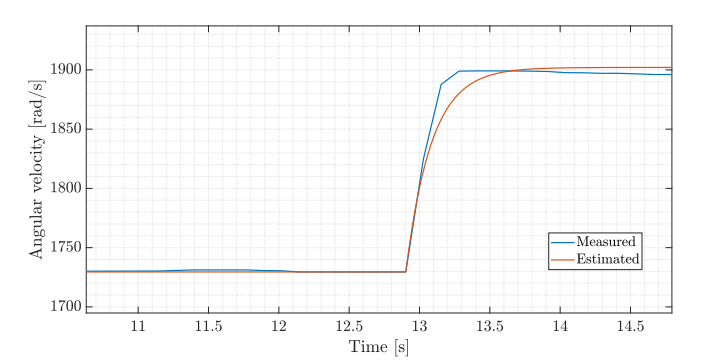
\includegraphics[width=0.75\linewidth]{Images/Motor dynamic response.png}
    \caption{Motor dynamic response, measured and identified response, motor powered from DC power supply at 14.8 V, motor for forward flight $KDE2304XF-2350$, 5x4.5 inch, 2 blades bullnose propeller.}
    \label{fig:Motor dynamic response}
\end{figure}

\begin{figure}
    \centering
    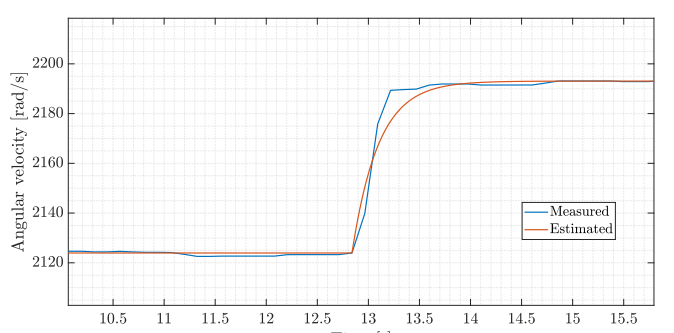
\includegraphics[width=0.75\linewidth]{Images/Motor dynamic response2.png}
    \caption{Motor dynamic response, measured and identified response, motor powered from DC power supply at 14.8 V, motor for vertical flight $KDE2315XF-2050$, 5x4.5 inch, 2 blades bullnose propeller.}
    \label{fig:Motor dynamic response2}
\end{figure}

\begin{figure}
    \centering
    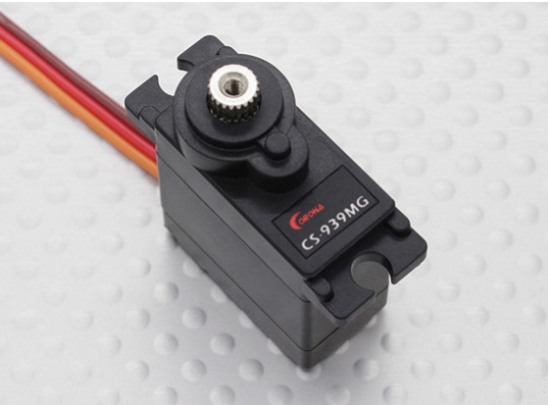
\includegraphics[width=0.5\linewidth]{Images/Corona 939 Metal Gear.png}
    \caption{Corona 939 Metal Gear}
    \label{fig:Corona 939 Metal Gear}
\end{figure}

\subsubsection{Gravity Elements}
To account for the influence of gravity force, a gravity element needs to be added. The 3D drive caller \textit{gravity\_acceleration} represents the gravity acceleration in the global reference frame.
This drone works below 100m, so the change of gravity acceleration with height could be neglected. The gravity acceleration is set to -9.81 m/s in the global Z-axis direction.

\subsubsection{Output Elements}
Output elements facilitate inter-process communication and can use specific communication means based on the type of simulation they are used for. They can transmit various types of data. In this simulation, the Stream output element is employed as a special element responsible for sending output to external processes via either \textit{local} or \textit{inet} sockets during batch or real-time simulations. It's worth noting that this topic is under development, so expect frequent changes, and please do not rely too heavily on backward compatibility. 

The Stream output allows MBDyn to send streamed outputs to remote processes during both batch and real-time simulations, using sockets either in the \textit{local} or \textit{inet} namespace. If the simulation runs in real-time using RTAI, RTAI mailboxes are used instead. The socket port is set to 10011, and \textit{send first} is enabled so that the control system could receive necessary airframe status information promptly. To obtain real-time flight status, including position, velocity, Euler angles, and angular velocity, data can be sourced from the \textit{MassCenter} node and its aircraft instruments. Additionally, to capture the force and moment acting on the center of mass, a total joint is utilized to link the \textit{MassCenter} node with the root. This arrangement allows for the representation of the rigid body within the root node, thereby facilitating the presentation of the force and moment acting on the center of mass through this joint. The total output information is shown in table \ref{tab:output element}.

\begin{table}
    \centering
    \begin{tabular}{ccc}
    \hline
        Output information & Number of ports & Unit\\
    \hline
        Position in global frame & 3 & $m$ \\
        Velocity in global frame & 3 & $m/s$ \\
        Acceleration in global frame & 3 & $m/s^2$ \\
        Euler angle in body frame & 3 & $rad$ \\
        Euler rates in body frame & 3 & $rad/s$ \\
        Euler angular acceleration & 3 & $rad/s^2$ \\
        Quaternions & 4 & 1 \\
        airspeed & 1 & $m/s$ \\
        angle of attack & 1 & $rad$ \\
        angle of slip & 1  & $rad$ \\
        Velocity in body frame & 3  & $rad/s$ \\
        altitude & 1 & $m$ \\
        Forces acted on mass of center of drone in body frame & 3 & $N$ \\
        Torques acted on mass of center of drone in body frame & 3 & $N \cdot m$ \\
    \hline
    \end{tabular}
    \caption{Output Information}
    \label{tab:output element}
\end{table}

\subsection{MBDyn Model Verification}
To validate the accuracy of the MBDyn model simulation, tests were conducted at an airspeed of 22 m/s. The default condition was tested with the aircraft fixed on the ground, having null attitude angles and null control surface deflections. In an additional case, the aircraft was positioned at a pitch angle of 5 degrees, and each control surface (aileron, elevator, rudder) was deflected by 5 degrees. Additionally, a rolling rotation velocity of 0.1 degrees per second was applied.

Expected values were manually calculated based on the same conditions using MBDyn simulation. Aerodynamic coefficients for each element were obtained according to the deflection angles set in the simulation. The total force and moment acting on the mass center were then calculated using dynamic pressure and measurements related to the mass center of each part. The table \ref{tab:Comparison of expect value and simulated results} presents the results, including both the simulation and manual expected computation:

\begin{sidewaystable}[htbp]
\centering
\begin{tabular}{|l|c|c|c|c|c|c|}
\hline
\textbf{Condition} & \textbf{$F_{x}$ (N)} & \textbf{$F_{y}$ (N)} & \textbf{$F_{z}$ (N)} & \textbf{$M_{x}$ (m*N)} & \textbf{$M_{y}$ (m*N)} & \textbf{$M_{z}$ (m*N)} \\
\hline
default condition & expect & -5.13E+00 & 0.00E+00 & 1.24E+02 & 0.00E+00 & -3.88E-01 \\
& Simulation & -5.14E+00 & 0.00E+00 & 1.24E+02 & -1.78E-15 & -3.88E-01 \\
& Error & 0.36\% & 0.00\% & 0.39\% & 0.00\% & 0.04\% \\
\hline
Pitch (5°) & expect & -1.05E+01 & 0.00E+00 & 2.10E+02 & 0.00E+00 & 1.09E-01 \\
& Simulation & -1.05E+01 & 0.00E+00 & 2.10E+02 & 3.46E-15 & 1.04E-01 \\
& Error & 0.01\% & 0.00\% & 0.00\% & 0.00\% & 4.68\% \\
\hline
Aileron (5°) & expect & -5.11E+00 & 3.56E-13 & 1.23E+02 & -6.69E+00 & -3.87E-01 \\
& Simulation & -5.11E+00 & 3.56E-13 & 1.23E+02 & -6.69E+00 & -3.87E-01 \\
& Error & 0.00\% & 0.00\% & 0.00\% & 0.00\% & 0.00\% \\
\hline
Elevator (5°) & expect & -5.16E+00 & 0.00E+00 & 1.26E+02 & 0.00E+00 & 1.74E+00 \\
& Simulation & -5.12E+00 & 0.00E+00 & 1.23E+02 & -1.78E-15 & -1.44E+00 \\
& Error & 0.00\% & 0.00\% & 0.00\% & 0.00\% & 0.00\% \\
\hline
Rudder (5°) & expect & -5.14E+00 & -3.54E-01 & 1.24E+02 & 3.15E-02 & -3.88E-01 \\
& Simulation & -5.14E+00 & -3.54E-01 & 1.24E+02 & 3.15E-02 & -3.88E-01 \\
& Error & 0.00\% & 0.00\% & 0.00\% & 0.00\% & -0.05\% \\
\hline
Rolling (0.1°/s) & expect & -5.14E+00 & 0.00E+00 & 1.24E+02 & -5.80E-02 & -3.88E-01 \\
& Simulation & -5.13E+00 & -1.08E+00 & 1.24E+02 & -5.62E-02 & -4.13E-01 \\
& Error & 0.36\% & 0.00\% & 0.39\% & 3.22\% & -6.08\% \\
\hline
\end{tabular}
\caption{Comparison of expect value and simulated results}
\label{tab:Comparison of expect value and simulated results}
\end{sidewaystable}

Comparison of the desired force and moment acting on the mass center with the simulation results reveals significant differences in the moment along the y-axis. This discrepancy may be attributed to errors in the main wing data or calculations. However, the results for all other metrics generally align with expectations. In the rolling movement section, the force and moment are affected by the non-linear relationship with the angle of attack. Consequently, there is a notable error compared to the simulation results, although it remains consistent with the manual computation. Figure \ref{fig:Force and moment monitored in clamp joint} illustrates the simulation results for force and moment in the global frame. Signals in the figure exhibit negligible noise caused by the simulation algorithm, which is lower than the error tolerance.

\begin{figure}[htbp]
    \centering
    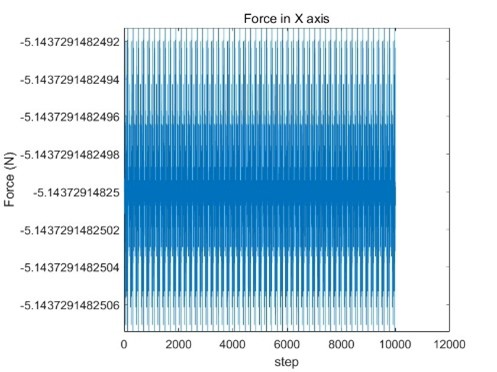
\includegraphics[width=0.45\textwidth]{Images/Vertify init/Picture1.jpg}
    \hfil
    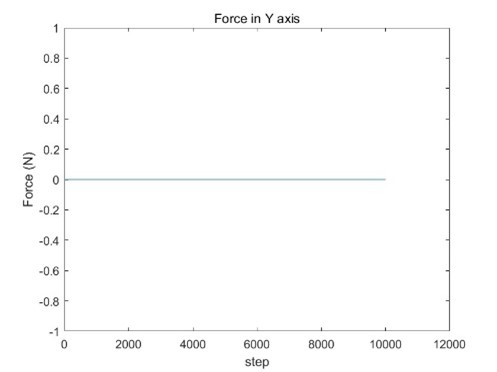
\includegraphics[width=0.45\textwidth]{Images/Vertify init/Picture2.jpg}
    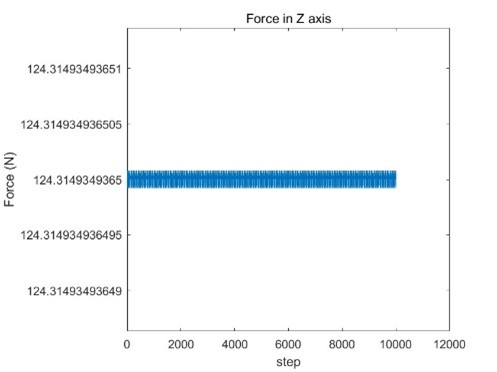
\includegraphics[width=0.45\textwidth]{Images/Vertify init/Picture3.jpg}
    \hfil
    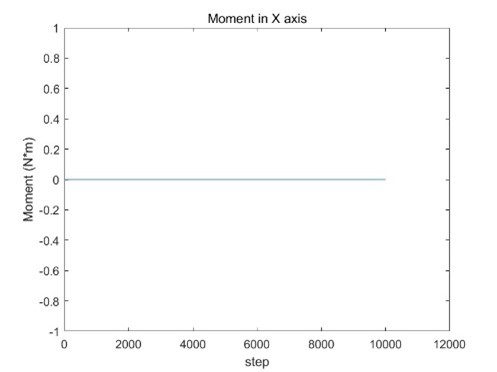
\includegraphics[width=0.45\textwidth]{Images/Vertify init/Picture4.jpg}
    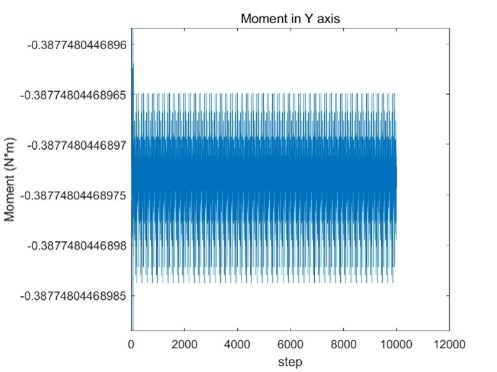
\includegraphics[width=0.45\textwidth]{Images/Vertify init/Picture5.jpg}
    \hfil
    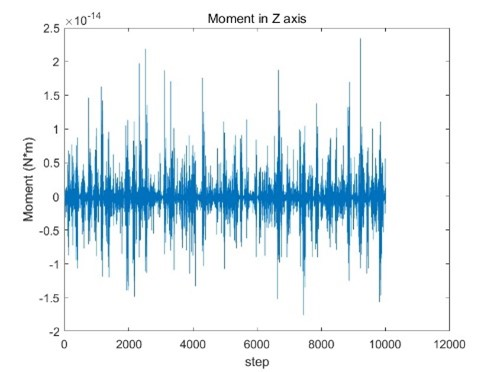
\includegraphics[width=0.45\textwidth]{Images/Vertify init/Picture6.jpg}
    \caption{Force and moment signal noise monitored in \textit{MassCenter} clamp joint}
    \label{fig:Force and moment monitored in clamp joint}
\end{figure}
